\documentclass[12pt]{article}

\usepackage{graphicx} % Required for inserting images
\usepackage[margin=2cm]{geometry}
\usepackage{booktabs}
\usepackage{amsmath}
\usepackage{amssymb}

\usepackage{hyperref}
\urlstyle{same}

\graphicspath{{./images/}}

\title{Predicting Heart Disease Diagnoses via Machine Learning Classification Models}
\author{Henry Mull}
\date{}

\begin{document}

\maketitle

% ============
% Requirements
% ============

% - Main objective of the analysis that specifies whether your model will be focused
%   on prediction or interpretation and the benefits that your analysis provides to
%   the business or stakeholders of this data.

% - Brief description of the data set you chose, a summary of its attributes, and an
%   outline of what you are trying to accomplish with this analysis.

% - Brief summary of data exploration and actions taken for data cleaning and
%   feature engineering.

% - Summary of training at least three different classifier models, preferably of
%   different nature in explainability and predictability. For example, you can 
%   start with a simple logistic regression as a baseline, adding other models or 
%   ensemble models. Preferably, all your models use the same training and test 
%   splits, or the same cross-validation method.

% - A paragraph explaining which of your classifier models you recommend as a final 
%   model that best fits your needs in terms of accuracy and explainability.

% - Summary Key Findings and Insights, which walks your reader through the main 
%   drivers of your model and insights from your data derived from your classifier 
%   model.

% - Suggestions for next steps in analyzing this data, which may include suggesting 
%   revisiting this model after adding specific data features that may help you 
%   achieve a better explanation or a better prediction.

\section*{Introduction}

% - Main objective of the analysis that specifies whether your model will be focused
%   on prediction or interpretation and the benefits that your analysis provides to
%   the business or stakeholders of this data.

% - Brief description of the data set you chose, a summary of its attributes, and an
%   outline of what you are trying to accomplish with this analysis.

The data set analysed and described below contains health information from 918 
patients and their heart disease diagnoses. As the diagnosis is a simply binary 
assignment, the models tested are various classification models which predict 
whether a patient has heart disease. While they will primarily focus on prediction, 
gaining insight into the causes of heart disease will also be equally important. 
Being able to accurately predict heart disease in new patients could drastically 
speed up diagnosis and would allow for those who were misdiagnosed to get the 
treatment they need, potentially saving lives. 

Contained in the data set are 11 columns which are a mix of numeric and categorical 
data. The columns and their descriptions are summarized below:
\begin{center}
    \begin{tabular}{l l p{4.5in}}
        \toprule
        Name & Type & Description \\
        \midrule
        Age & Numeric & Age of the patient \\
        Sex & Categorical & Sex of the patient; M: Male, F: Female \\
        ChestPainType & Categorical & Type of chest or heart pain; ASY: asymptomatic, TA: Typical angina, ATA: atypical angina, NAP: non-angina pain \\
        RestingBP & Numeric & Blood pressure when at rest (mm Hg) \\
        Cholesterol & Numeric & Cholesterol level (mg/dl) \\
        FastingBS & Categorical & Blood sugar when fasting; 0: $\leq$120 mg/dl, 1: $>$120 mg/dl \\
        RestingECG & Categorical & Resting electrocardiograph results; Normal , ST: ST-T wave abnormality, LVH: probable or definite left ventricular hypertrophy \\
        MaxHR & Numeric & Maximum heart rate \\
        ExerciseAngina & Catagorical & Exercised-induced chest or heart pain; 0: No, 1: Yes \\
        Oldpeak & Numeric & Exercise-induced ST depression \\
        ST\_Slope & Catagorical & Slope of exercise ST segment; Flat, Up: slopes up, Down: slopes down \\
        \bottomrule
    \end{tabular}    
\end{center}    
The final column, whose values  of the data set is ``HeartDisease'' and is either 0 for a 
negative diagnosis or 1 for a positive one. The full data set was obtained on Kaggle at 
\url{https://www.kaggle.com/datasets/amirmahdiabbootalebi/heart-disease/data}.

\section*{Exploratory Data Analysis and Preprocessing}

% - Brief summary of data exploration and actions taken for data cleaning and feature engineering.

An initial examination of the data was performed using a Seaborn pairplot. The mixed plots 
show that there is significant overlap between the positive and negative diagnoses in plot. 
Additionally, there appears to be low correlation between the features other that between 
age and maximum heart rate which has a negative relationship as expected. On the diagonal, 
the histograms generally have normal-looking distributions; however, one possible source of 
concern is that there appears to be data points which have a cholesterol reading of 0. Upon 
closer inspection, there appears to be one data point which also has a 0 for the resting 
blood pressure, which hopefully for the patient was simply an oversight. These points 
account for 172 of the 918 total samples and so they represent a significant portion of the 
data. By removing these points, the score metrics decrease by several percentage points 
across the board, thus they have been left in. 

Because there were different data types and scales, the data was first examined for any 
necessary preprocessing. For the numeric data, calculating the skewness showed that there 
was unlikely a need for transforming the data, expect possibly for Oldpeak which had a 
skewness of 1.02. However, because of the presence of negative values, with the fact that it
is not an extreme skew value, it was left alone. The numeric columns were then scaled using 
min-max scaling to bring all of the values between 0 and 1. Finally, the categorical 
features were one-hot encoded, where the binary categories were transformed into a single 
column of 0's and 1's, and the features with multiple categories became $n-1$ new features 
with the first category dropped.

\section*{Model Training}

% - Summary of training at least three different classifier models, preferably of different 
%   nature in explainability and predictability. For example, you can start with a simple 
%   logistic regression as a baseline, adding other models or ensemble models. Preferably, 
%   all your models use the same training and test splits, or the same cross-validation 
%   method.

The data set was separated into training and test sets using the \texttt{train\_test\_split}
method contained in \texttt{sklearn}. The test set contained $\sim10\%$ of the set and was 
stratified to ensure a similar distribution between sets which was $55\%$ and $45\%$ for the
positive and negative diagnoses, respectively. Due to the similar class sizes for the data, 
it is likely unnecessary to use class weighting, oversample, or undersampling. 

Most models utilised hyperparameters which were optimized through \texttt{sklearn}'s built 
in cross-validation variations of the models or the \texttt{GridSearchCV} object. A summary 
of the models and their final hyperparameters is shown below:
\begin{center}
    \begin{tabular}{l l l}
        \toprule
        Model & Abbr. & Hyperparameters \\
         \midrule
        Logistic Regression & logr & C: $0.35938137$; penalty: l2 \\
        Support Vector Machine & svm & C: $1.0$; kernel: rbf \\
        K-nearest Neighbors & knn & n\_neighbors: 7 \\
        Decision Tree Classifier & dtc & max\_depth: 3; max\_features: 11 \\
        Random Forest Classifier & rfc & n\_estimators: 80, max\_depth: 10; max\_features: 1 \\
        Bagging Classifier & bag & n\_estimators: 11; max\_features: 7 \\
        Extra Tress Classifier & etc & n\_estimators: 90, max\_depth: 13; max\_features: 1\\
        AdaBoost Classifier & abc & learning\_rate: 0.1; n\_estimators: 70 \\
         \bottomrule
    \end{tabular}    
\end{center}
Each model was trained using the scaled training data, and the accuracy, precision, recall, 
and f1 metrics using the test set were collected. Overall, the lowest score was 0.79 which 
was the precision of the bagging model, while the highest score was 0.88 and was the recall 
score of the logistic regression, k-nearest neighbors, and bagging models. All of the 
scoring metrics for each model are shown in the graph below. 
\begin{figure}[ht]
    \centering
    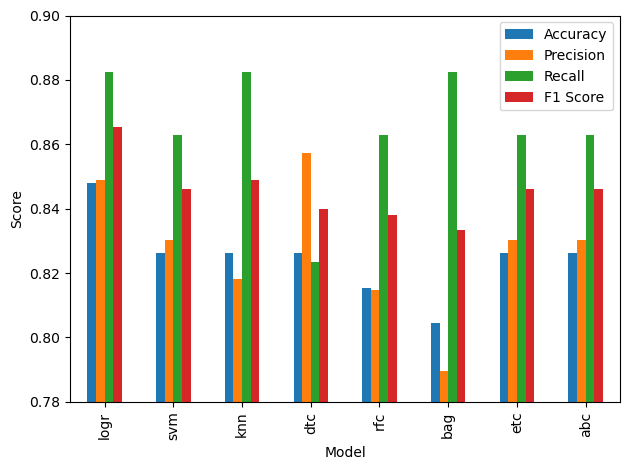
\includegraphics[height=2.5in]{test_plot.png}
\end{figure}

% - A paragraph explaining which of your classifier models you recommend as a final model 
%   that best fits your needs in terms of accuracy and explainability.

From these results, the best performing model is the logistic regression model. It 
consistently ranks at or near the top of the models for each performance metric. 
Additionally, it offers high interpretability as the coefficients from the model give a 
simple indication of how the features positively or negatively affect the classification. 
Many of the coefficients have expected behavior, such as being positively correlated to age 
and the presence of exercise-induced chest pain, and negatively correlated to asymptomatic 
features; however, other features behave contrary to expectations, like cholesterol which is
negatively correlated. This could be an indication of either a feature which requires 
further study to understand the relationship or a feature which needs additional or cleaner 
data. The k-nearest neighbors model had the next highest set of scores, however it would be 
much more difficult to offer explanations, especially as the pairplot demonstrated for all 
of the features that there was significant overlap between the positive and negative 
diagnoses. Because of the k-nearest neighbors algorithm, it would also be more difficult to 
expand the model relative to logistic regression. If the training sets were greatly expanded
as more data is collected, the k-nearest neighbors model would take increasingly longer to 
test new cases.

\section*{Summary}

% - Summary Key Findings and Insights, which walks your reader through the main drivers of 
%   your model and insights from your data derived from your classifier model.

Logistic regression provided the highest performing model according to the accuracy, 
precision, recall, and f1 scoring metrics. Many of the models provided similar levels of 
performance, with many scores being in the range of 0.82 to 0.86. The coefficients provided 
by the logistic regression model offer easily understandable insights to the correlation of 
each of the features and the final diagnosis. One such insight is the negative correlation 
between heart disease and being female, which is well-understood and documented. 
Additionally, having exercise-induced angina, old age, high blood sugar and pressure, and 
ECG abnormalities are all positively correlated, while asymptomatic features and max heart 
rate are negatively correlated. 

% - Suggestions for next steps in analyzing this data, which may include suggesting 
%   revisiting this model after adding specific data features that may help you achieve a 
%   better explanation or a better prediction.

In examining the incorrect predictions of the model, it becomes obvious that there are 
specific samples that are consistently missed by all or most models. There were eight 
samples which were incorrectly assigned, whether a false positive or negative, by every 
single model. If the samples which were mislabeled by at least 6 of the models are 
considered, that accounts for 38\% of the test set. Because of this high frequency of 
incorrect assignments by multiple models, it is possible that this data set needs 
additional features to account for this additional variance. With new features, new data 
points would also be helpful in finding new patters as there were fewer that 1000 data 
points in the original data set. The existing data would also likely benefit from further 
cleaning or updating, as there are a significant number of points which have report a 
cholesterol level of 0, and fixing this may help resolve the issue with the negative 
correlation of the current model.

\end{document}
